
%(BEGIN_QUESTION)
% Copyright 2010, Tony R. Kuphaldt, released under the Creative Commons Attribution License (v 1.0)
% This means you may do almost anything with this work of mine, so long as you give me proper credit

Denne forbrenningsoppvarmede ovnen bruker to regulatorer: én for å regulere luftstrøm inn til brenneren, og én for å regulere lufttrykket inne i ovnen. Luftstrømsregulering er viktig for riktig oppvarming, og lufttrykksregulering er viktig for å hindre lekkasje rundt døråpninger og andre åpninger i ovnen:

$$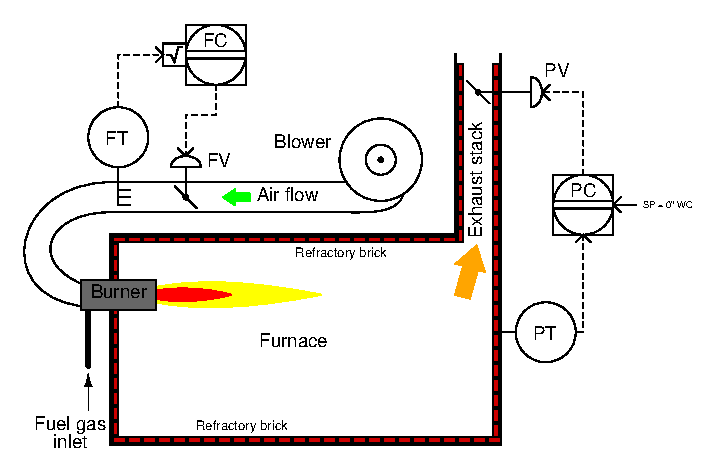
\includegraphics[width=15.5cm]{i01554x01.eps}$$

Anta at du en dag får beskjed om et problem med denne ovnen: flammer observeres rundt kantene på dørene inn til ovnen mens den er i drift.

Identifiser sannsynligheten for hver spesifiserte feil for denne prosessen. Vurder hver feil én om gangen (dvs. ingen samtidige feil), og avgjør om hver feil alene kan forklare {\it alle} målinger og symptomer i prosessen.

% No blank lines allowed between lines of an \halign structure!
% I use comments (%) instead, so that TeX doesn't choke.

$$\vbox{\offinterlineskip
\halign{\strut
\vrule \quad\hfil # \ \hfil & 
\vrule \quad\hfil # \ \hfil & 
\vrule \quad\hfil # \ \hfil \vrule \cr
\noalign{\hrule}
%
% First row
{\bf Feil} & {\bf Mulig} & {\bf Umulig} \cr
%
\noalign{\hrule}
%
% Another row
Blåserhastighet for høy &  &  \cr
%
\noalign{\hrule}
%
% Another row
FC i manuell modus &  &  \cr
%
\noalign{\hrule}
%
% Another row
PC i manuell modus &  &  \cr
%
\noalign{\hrule}
%
% Another row
FT litt feilkalibrert (viser for mye strømning) &  &  \cr
%
\noalign{\hrule}
%
% Another row
FT litt feilkalibrert (viser for lite strømning) &  &  \cr
%
\noalign{\hrule}
%
% Another row
PT litt feilkalibrert (viser for høyt trykk) &  &  \cr
%
\noalign{\hrule}
%
% Another row
PT litt feilkalibrert (viser for lavt trykk) &  &  \cr
%
\noalign{\hrule}
} % End of \halign 
}$$ % End of \vbox

Til slutt: identifiser den {\it neste} diagnostiske testen eller målingen du ville utført på dette systemet. Forklar hvordan resultatet/resultatene av denne testen eller målingen hjelper deg å snevre inn plassering og/eller type feil.

\vskip 20pt \vbox{\hrule \hbox{\strut \vrule{} {\bf Forslag til sokratisk diskusjon} \vrule} \hrule}

\begin{itemize}
\item{} Hva indikerer ISA-symbolene om designen til begge reguleringsventilene?
\item{} Hva indikerer ISA-symbolene om plasseringen av de to regulatorene?
\item{} Hvilken type strømningsmåler brukes her for å måle forbrenningsluftstrøm?
\end{itemize}

\underbar{file i01554}
%(END_QUESTION)





%(BEGIN_ANSWER)

% No blank lines allowed between lines of an \halign structure!
% I use comments (%) instead, so that TeX doesn't choke.

$$\vbox{\offinterlineskip
\halign{\strut
\vrule \quad\hfil # \ \hfil & 
\vrule \quad\hfil # \ \hfil & 
\vrule \quad\hfil # \ \hfil \vrule \cr
\noalign{\hrule}
%
% First row
{\bf Feil} & {\bf Mulig} & {\bf Umulig} \cr
%
\noalign{\hrule}
%
% Another row
Blåserhastighet for høy &  & $\surd$ \cr
%
\noalign{\hrule}
%
% Another row
FC i manuell modus & (avhenger) &  \cr
%
\noalign{\hrule}
%
% Another row
PC i manuell modus & $\surd$ &  \cr
%
\noalign{\hrule}
%
% Another row
FT litt feilkalibrert (viser for mye strømning) &  & $\surd$ \cr
%
\noalign{\hrule}
%
% Another row
FT litt feilkalibrert (viser for lite strømning) &  & $\surd$ \cr
%
\noalign{\hrule}
%
% Another row
PT litt feilkalibrert (viser for høyt trykk) &  & $\surd$ \cr
%
\noalign{\hrule}
%
% Another row
PT litt feilkalibrert (viser for lavt trykk) & $\surd$ &  \cr
%
\noalign{\hrule}
} % End of \halign 
}$$ % End of \vbox

Om FC i manuell modus kan forklare dette ovnsproblemet eller ikke, avhenger av om avgasspjeldet har kapasitet til å ventilere nok avgass til å holde settpunkt selv med for høy inngående luftstrøm. Hvis ja, vil FC i manuell modus {\it ikke} forklare problemet. Hvis nei, {\it kan} FC i manuell modus forklare problemet.

%(END_ANSWER)





%(BEGIN_NOTES)

En god ``neste test'' vil være å se på PV-visningen på trykkregulatoren, for å se om regulatoren ``tror'' at PV faktisk er på settpunkt, når vi vet at den tydelig ikke er det (fordi flammer slipper ut rundt dørkantene).




\filbreak \vskip 20pt \vbox{\hrule \hbox{\strut \vrule{} {\bf Virtuell feilsøking} \vrule} \hrule}

\noindent
{\bf Predikere effekten av en gitt feil:} presenter hver av følgende feil for studentene, én om gangen, og la dem kommentere alle effektene hver feil vil gi.

\begin{itemize}
\item{}
\item{}
\item{}
\end{itemize}


\vskip 10pt


\noindent
{\bf Identifisere mulige/umulige feil:} presenter symptomer for studentene og la dem deretter avgjøre om en rekke foreslåtte feil kan forklare alle symptomene, med forklaring av {\it hvorfor} eller {\it hvorfor ikke} for hver foreslåtte feil:

\begin{itemize}
\item{} Symptom: {\it }
\item{}  -- {\bf Ja/Nei}
\item{}  -- {\bf Ja/Nei}
\item{}  -- {\bf Ja/Nei}
\end{itemize}


\vskip 10pt


\noindent
{\bf Bestemme nytten av gitte diagnostiske tester:} presenter symptomer for studentene og foreslå deretter følgende diagnostiske tester én etter én. Studentene vurderer verdien av hver test, og avgjør om den vil gi nyttig informasjon (dvs. fortelle oss noe vi ikke allerede vet). Studentene bestemmer hva ulike resultater av hver test vil indikere om feilen, hvis noe:

\begin{itemize}
\item{} Symptom: {\it }
\item{}  -- {\bf Ja/Nei}
\item{}  -- {\bf Ja/Nei}
\end{itemize}


\vskip 10pt


\noindent
{\bf Diagnostisere en feil basert på gitte symptomer:} forestill deg at ??? feiler ??? i dette systemet (ikke avslør feilen for studentene!). Presenter operatørens observasjon(er) for studentene, la dem vurdere mulige feil og diagnostiske strategier, og fortell dem deretter resultatene av testene de foreslår basert på følgende symptomer, helt til de har identifisert type og plassering av feilen korrekt:

\begin{itemize}
\item{} Operatørobservasjon: {\it }
\item{}
\item{}
\end{itemize}

%INDEX% Process: combustion furnace

%(END_NOTES)

